This section shows how we extend the Sparse Conditional
Constant propagation (SCC) algorithm from \cite{WZ91} so as to enable
constant propagation through array elements in conjunction with 
unreachable code elimination.
Section~\ref{sec:scc:flags} outlines the lattice variables
for {\it executable flags} used by our algorithm, and also shows
how the lattice value of a $\Phi$ operator is evaluated in the
presence of executable flags.
Section~\ref{sec:scc:alg} contains a description of our extended
SCC algorithm that enables constant propagation through scalars and
array elements.

\subsection{Lattice values of executable flags for nodes and edges}\label{sec:scc:flags}


As in the SCC algorithm in \cite{WZ91},
our array conditional constant propagation
algorithm maintains executable flags associated with each node and
each edge in the CFG. Flag $X_{ni}$ indicates
whether node $n_i$ may be executed, and $X_{ei}$ indicates whether
edge $e_i$ may be traversed.  The lattice value of an execution
flag is either $\No$ or $\Maybe$, corresponding to
unreachable code and reachable code respectively.
The lattice ordering for these two elements is $\No \sqsupset \Maybe$,
so we can think of $\No$ as $\top$ (top) and $\Maybe$ as $\bot$ (bottom).
The lattice
value for an
execution flag is initialized to $\No$, and can be lowered to $\Maybe$
in the course of the constant propagation algorithm.
In practice, control dependence identities can be used to reduce the number of executable flag variables in the data-flow equations \eg\ a single flag can be used for all CFG nodes that are control equivalent.  For the sake of
simplicity, we ignore such optimizations in this chapter.


As discussed in section~\ref{sec:arrayssa}, 
the executable flags serve as an approximation for @ variables
from full Array SSA form when computing the lattice value
for a $\Phi$ operator in the case of conditional constant propagation.
Recall that the
$\L_{\phi}$ function for a control $\phi$
was defined in section~\ref{sec:sc} by the  join function,
$\L_{\phi}(\L(A_2),\L(A_1)) =\ \L(A_1) \sqcap
\L(A_2)$.  For the extended SCC algorithm described in this section,
we use the definition of $\L_{\Phi}$ shown
in figure~\ref{fig:phi}.  This definition uses executable flags
$X_{e1}$ and $X_{e2}$, where $e1$ and $e2$ are the incoming control-flow edges for the $\Phi$ function.  Thus, the lattice values of the
executable flags $X_{e1}$ and $X_{e2}$
are used as compile-time approximations of 
@ variables $@k_1$ and $@k_2$ from the
full Array SSA form.


\begin{figure}%[p]
\begin{center}
\begin{tabular}{|l||c|c|c|}
\hline
$\L(k_3)$ & $X_{e2} = \No$ & $X_{e2} = \Maybe $  \\
\hline \hline
$X_{e1} = \No$ & $\top$ & $\L(k_2)$   \\
\hline
$\X_{e1} = \Maybe$ & $\L(k_1)$ & $\L(k_1) \sqcap \L(k_2)$    \\
\hline
\end{tabular}
\end{center}
\caption{$\L(k_3) := \L_{\Phi}(\L(k_1), X_{e1}, \L(k_2), X_{e2} )$, where execution flags $X_{e1}$ and
$X_{e2}$ control the selection of $k_1$ and $k_2$ respectively}
\label{fig:phi}
\end{figure}

\begin{figure}%[p]
\begin{tabular}{lr}
\begin{minipage}{3.75in}
{\bf Definition of join operator, $X_n = X_{e1} \sqcap X_{e2}$:}

\medskip

\begin{tabular}{|l||c|c|}
\hline
$X_n$ & $X_{e2} = \No$ & $X_{e2} = \Maybe$  \\
\hline \hline 
$X_{e1} = \No$ & $\No$ & $\Maybe$  \\
\hline
$X_{e1} = \Maybe$ & $\Maybe$ & $\Maybe$  \\
\hline
\end{tabular}
\end{minipage}
&
\begin{minipage}{1.0in}
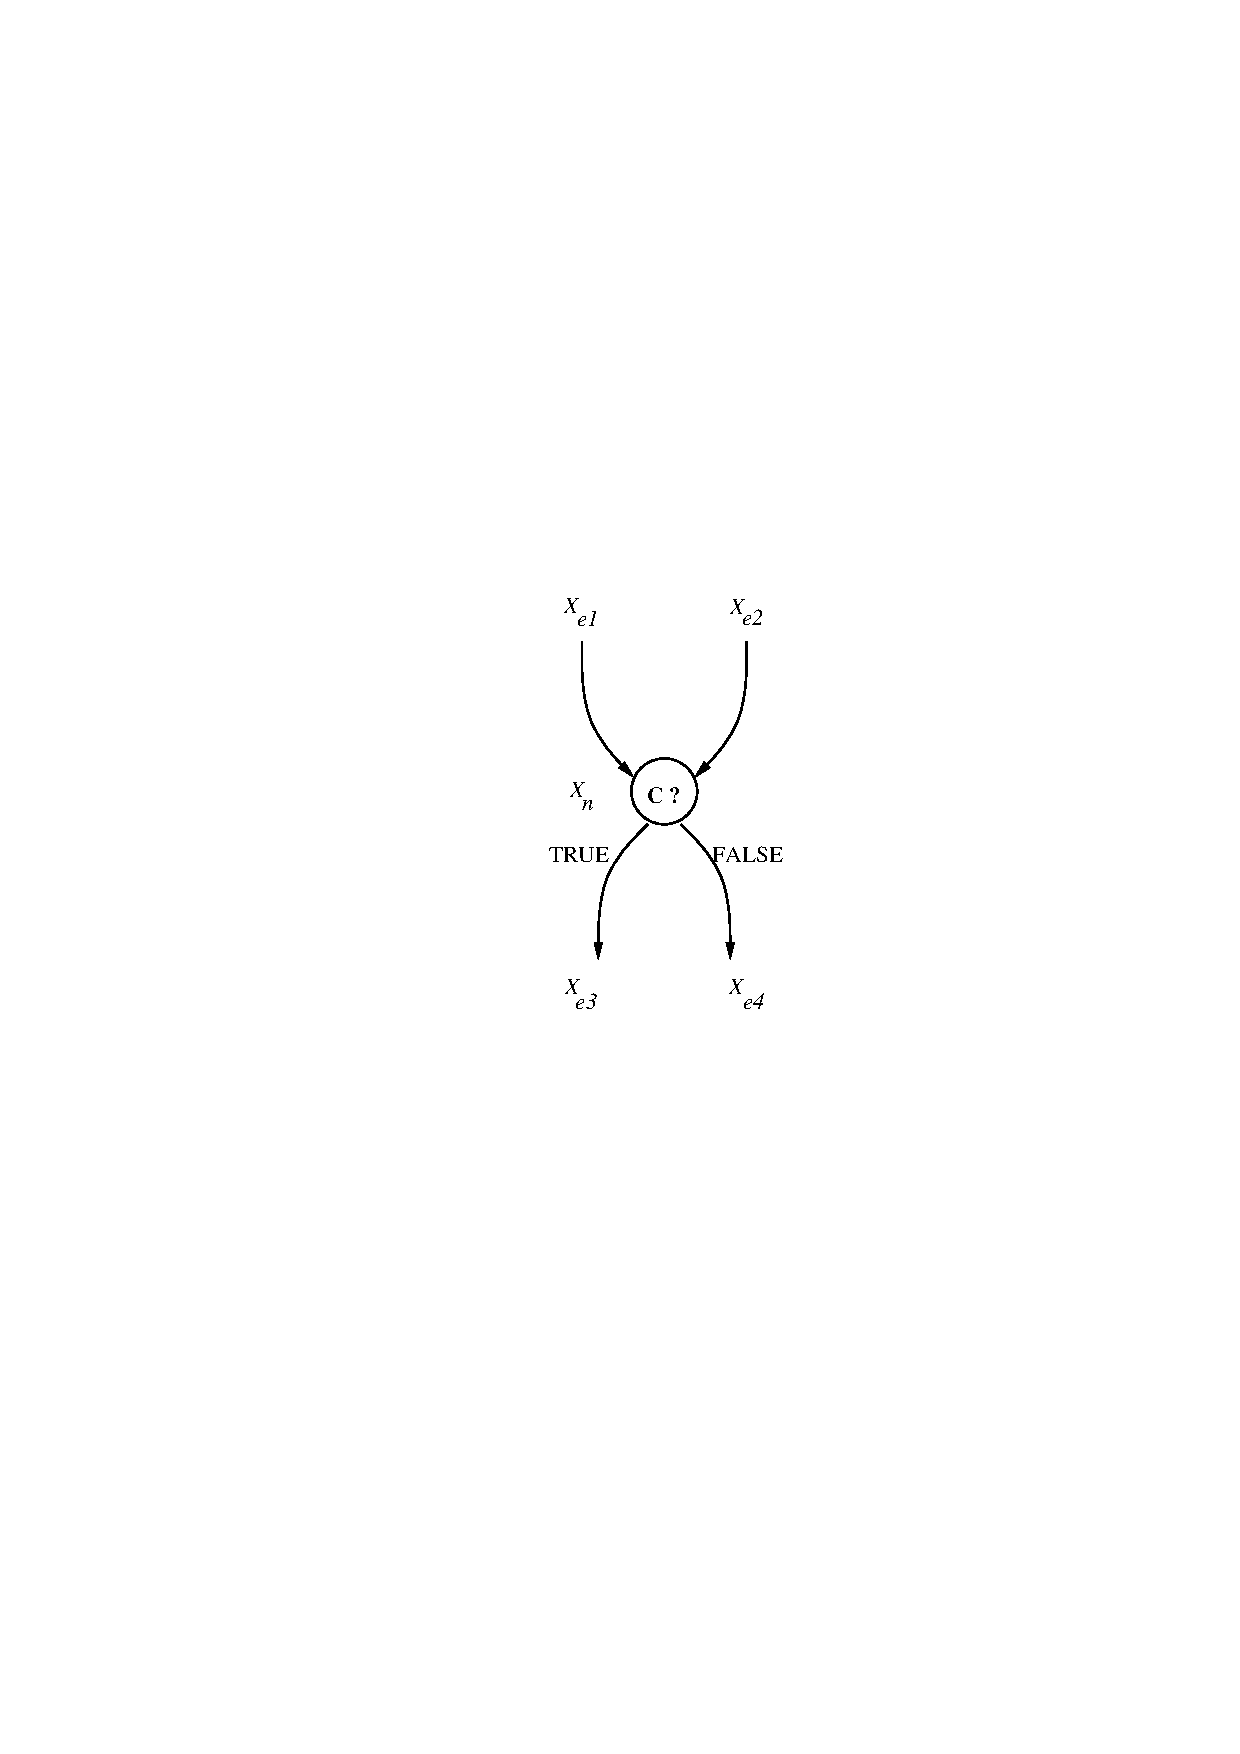
\includegraphics[width=0.1in]{branch.pdf}
\end{minipage}
\end{tabular}

\bigskip
\bigskip

{\bf Definition of true operator for branch condition $C$,\\
$X_{e3} = \L_{\T}(X_n,\L(C))$:}

\medskip

\begin{tabular}{|l||c|c|c|c|}
\hline
$X_{e3}$ & $\L(C) = \top$ & $\L(C) = \True$ & $\L(C) = \False$ & $\L(C) = \bot$ \\
\hline \hline
$X_n = \No$ & $\No$ & $\No$ & $\No$ & $\No$ \\
\hline
$X_n = \Maybe $ & $\No$ & $\Maybe$ & $\No$ & $\Maybe$ \\
\hline
\end{tabular}

\bigskip
\bigskip

{\bf
Definition of false operator for branch condition $C$,\\
$X_{e4} = \L_{\F}(X_n, \L(C))$:}

\medskip

\begin{tabular}{|l||c|c|c|c|}
\hline
 $X_{e4}$ & $\L(C) = \top$ & $\L(C) = \True$ & $\L(C) = \False$ & $\L(C) = \bot$ \\
\hline \hline
$X_n = \No$ & $\No$ & $\No$ & $\No$ & $\No$ \\
\hline
$X_n = \Maybe$ & $\No$ & $\No$ & $\Maybe$ & $\Maybe$ \\
\hline
\end{tabular}
\caption{Executable flag mappings for join operator \protect{$(\sqcap)$},
true operator \protect{$(\L_{\T})$}, and false operator \protect{$(\L_{\F})$}}
\label{fig:mappings}
\end{figure}

\REM{
This approach is a compromise between the full Array SSA form on the
one hand and partial Array SSA form on the other.  Full Array SSA form
relies on exact control-flow information available at runtime to
support an exact $\Phi$ functions. Partial Array SSA as described for
use in SC presented in section~\ref{sec:sc} uses no flow information.
Here, for SCC, the flow information is available statically but is
coarse distinguishing only between edges that are never taken and
those that might be taken.
}

The executable flag of a node is computed from the executable flags
of its incoming edges. The executable flag of an edge is computed from
the executable flag of its source node and knowledge of the branch condition
variable used to determine the execution path from that node.
These executable flag mappings are summarized in figure~\ref{fig:mappings}
for  a node $n$ with two incoming edges, $e1$ and $e2$, and two 
outgoing edges, $e3$ and $e4$. The first
function table in figure~\ref{fig:mappings} defines
the {\it join operator}
$\sqcap$ on executable flags
such that $X_n = X_{e1} \sqcap X_{e2}$.  We 
introduce a {\it true operator}
$\L_{\T}$ and a {\it false operator} $\L_{\F}$ on lattice values
such that $X_{e3} = \L_{\T}(X_n,\L(C))$
and $X_{e4} = \L_{\F}(X_n,\L(C))$.  Complete function tables for the $\L_{\T}$ and
$\L_{\F}$ operators are also shown in figure~\ref{fig:mappings}.
Note that all three function tables are monotonic with respect to
their inputs.


Other cases for mapping a node $X_n$ value to the $X_e$ values of its
outgoing edges can be defined similarly.  If $n$ has exactly one
outgoing edge $e$, then $X_e = X_n$.  If node $n$ has more than two outgoing edges
then the mapping for each edge is similar to the $\L_{\T}$ and $\L_{\F}$
operators.



\REM
{
\begin{figure}%[p]

%\medskip
\begin{center}
\begin{tabular}{|l||c|c|c|c|}
\hline
$X_n$ & $X_{e2} = \top$ & $X_{e2} = \True$ & $X_{e2} = \False$ & $X_{e2} = \bot$ \\
\hline \hline
$X_{e1} = \top$ & $\top$ & $\True$ & $\top$ & $\True$ \\
\hline
$X_{e1} = \True$ & $\True$ & $\True$ & $\True$ & $\True$ \\
\hline
$X_{e1} = \False$ & $\top$ & $\True$ & $\False$ & $\bot$ \\
\hline
$X_{e1} = \bot$ & $\True$ & $\True$ & $\bot$ & $\bot$ \\
\hline
\end{tabular}
\end{center}
\caption{Definition of Union over lattice values}

\label{fig:union}
\end{figure}

\begin{figure}

\begin{center}
\begin{tabular}{|l||c|c|c|c|}
\hline
$X_n$ & $X_{e2} = \top$ & $X_{e2} = \True$ & $X_{e2} = \False$ & $X_{e2} = \bot$ \\
\hline \hline
$X_{e1} = \top$ & $\top$ & $\True$ & $\top$ & $\True$ \\
\hline
$X_{e1} = \True$ & $\True$ & $\True$ & $\True$ & $\True$ \\
\hline
$X_{e1} = \False$ & $\top$ & $\True$ & $\False$ & $\bot$ \\
\hline
$X_{e1} = \bot$ & $\True$ & $\True$ & $\bot$ & $\bot$ \\
\hline
\end{tabular}
\end{center}

\caption{Full definition of join operator, $X_n = X_{e1} \sqcap X_{e2}$:}

\label{fig:full-join}
\end{figure}
}



\REM{

As a robustness check, here is the function table for $X_{n2} = X_{e3}
\sqcap X_{e4} = \$\L_{T}(X_{n1}, \L(C)) \sqcap \L_{\F}(X_{n1}, \L(C))$, which 
will need to be
computed for the degenerate case in which two edges $e3$ and $e4$ both
go from node $n1$ to node $n2$.

\begin{figure}

\begin{center}
\begin{tabular}{|l||c|c|c|c|}
\hline
$X_{n2}$ & $C = \top$ & $C = \True$ & $C = \False$ & $C = \bot$ \\
\hline \hline
$X_{n1} = \top$ & $\top$ & $\top$ & $\top$ & $\top$ \\
\hline
$X_{n1} = \True$ & $\top$ & $\True$ & $\True$ & $\True$ \\
\hline
$X_{n1} = \False$ & $\False$ & $\False$ & $\False$ & $\False$ \\
\hline
$X_{n1}  = \bot$ & $\False$ & $\bot$ & $\bot$ & $\bot$ \\
\hline
\end{tabular}
\end{center}

\caption{Robustness check}
\label{fig:robust}
\end{figure}

To evaluate the robustness of the above mapping, consider replacing
edges $e3$ and $e4$ by a single unconditional edge $e34$. In this
case $X_{n2} = X_{e34} = X_{n1}$.  There are only two cases in which
the above table differs from the identity mapping:

\begin{enumerate} 

\item $X_n = \True$ and $C = \top$\\ 

In this case, we would expect $X_d$ to equal $X_n = \True$,
but the value in the table is $\top$.  However, this difference does not
pose a problem because if node $n$ is executable then the final lattice
value for $C$ cannot be $\top$ on termination of the propagation
algorithm. 

\item $X_n = \True$ and $C = \bot$\\

In this case, we would expect $X_d$ to equal $X_n = \True$, but the
value in the table is $X_d = X_{e3} \sqcap X_{e4} = \bot \sqcap \bot =
\bot$.  This imprecision can be avoided by observing that $X_d = \True$
for both the $C = \True$ and $C = \False$ cases (when $X_n = \True$) and
thus concluding that $X_d$ must equal $\True$ when $C = \bot$. 

QUESTION: Even though this degenerate case can be handle by special-case
simplification of CFG edges, the above imprecision might lead to problems
elsewhere.  Should we try and avoid this
imprecision by instead using a three-valued lattice for $X$ and $X$
with values drawn from the set $\{ \top, \False, \bot \}$?

Notice that we compute the $\bot$ column, as described above, as the
union of the $\True$ column and the $\False$ column on the core 3 x 3
table. The result is $\True$ as shown. If instead we compute the $\bot$
column directly from the full 4 x 4 tables using the robustness check
formula the result is $\bot$, a less precise result. This is because,
although for each edge the execution flag for that edge can be both
$\True$ and $\False$, the values for the two paths are correlated so
that the result (the $\sqcap$ of the two flags) is always $\True$. 

Conjecture: delaying the union operation for $\bot$ maximizes precision.
is this true? how can we use this in the algorithm? likely to impact
algorithmic complexity?

\end{enumerate}
}




\subsection{Sparse Conditional Constant Propagation Algorithm}\label{sec:scc:alg}


\begin{figure}%[p]
\begin{center}
\begin{programa}
/* INITIALIZATION */ \\
\Ta {\bf for each} lattice variable $\L(v)$ {\bf do}\\
\Tb {\bf if} it is not possible that $\L(v)$ can be recognized as a constant\\
\Td at compile-time (\eg\ $v$ is a return value from an unknown call)\\
\Tb {\bf then}\\
\Tc $\L(v)\  \leftarrow\ \bot $\\
\Tb {\bf else}\\
\Tc $\L(v)\  \leftarrow\ \top $\\
\Tb {\bf end if}\\
\Ta {\bf end for}\\
\\
\Ta {\bf for each} node/edge executable flag $X$ {\bf do}\\
\Tb {\bf if} $X$ is the executable flag for the entry node {\bf then}\\
\Tc $X\ \leftarrow\ \Maybe$ /* NOTE: $\Maybe$ is the same as $\bot$ */\\
\Tb {\bf else}\\
\Tc $X\ \leftarrow\ \No$ /* NOTE: $\No$ is the same as $\top$ */\\
\Tc $\L(v)\  \leftarrow\ \top $\\
\Tb {\bf end if}\\
\Ta {\bf end for}\\
\\
\Ta Intialize {\it worklist} $\leftarrow$ an empty list\\
\Ta {\bf for each} equation $E$ {\bf do}\\
\Tb {\bf if} the RHS of equation $E$ has at least one term that is $\not= \; \top$\\
\Td  (\ie\ at least one term that is $\bot$ or contains a constant)\\
\Tb {\bf then}\\
\Tc  Insert equation $E$ into the {\it worklist}\\
\Tb{\bf end if}\\
\Ta {\bf end for}\\
 \\
/* FIXPOINT ITERATION */ \\
\Ta {\bf while} {\it worklist} is not empty {\bf do}\\
\Tb $E \leftarrow$ remove any equation from {\it worklist}\\
\Tb Recompute $\L(v)$, the LHS of equation $E$, based on the values of $E$'s RHS terms\\
\Tb {\bf if} the LHS of equation $E$ has changed {\bf then}\\
\Tc {\bf for each} equation $E'$ that uses $\L(v)$ in its RHS {\bf do}\\
\Td Insert equation $E'$ into {\it worklist}\\
\Tc {\bf end for}\\
\Tb {\bf end if}\\
\Ta {\bf end while} \\
\\
/* TERMINATION */\\
\Ta For each Array SSA variable $v$ such that $\L(v)$ contains a constant, transform the \\ 
\Ta program to replace each use of $v$ by a constant, if profitable to do so
\end{programa}
\end{center}
\caption{Sparse Conditional Constant propagation (SCC) algorithm for scalar and array variables}
\label{fig:scc-alg}
\end{figure}

Figure~\ref{fig:scc-alg} contains an outline of our conditional constant
propagation algorithm for scalar and array variables.  It is similar in
structure to the sparse constant propagation algorithm for scalars
and arrays presented in figure~\ref{fig:sc-alg} (section~\ref{sec:sc}),
but there are two significant differences:
\begin{enumerate}
\item The inputs to the conditional constant propagation algorithm
in figure~\ref{fig:scc-alg}
contain additional lattice variables and data-flow equations due
to the executable flags introduced in section~\ref{sec:scc:flags}.
\item The initialization in figure~\ref{fig:scc-alg}
has to take care to mark the executable flag for the entry 
block as reachable ($\Maybe$).
\end{enumerate}
Compared to the SCC algorithm in \cite{WZ91}, the major extensions in
the algorithm in figure~\ref{fig:scc-alg} are that it propagates constants
through array elements and that the use of data-flow equations make
it possible to combine this analysis with other analyses in the future.


\begin{figure}%[p]
\begin{center}
\begin{tabular}{lcr}
\begin{minipage}{1.5in}
\begin{programa}
\mbox{n1:}\Tb $i := 1$ \\
\Tb $C := i\ <\ n $\\
\Tb if $C$ then \\
\mbox{n2:}\Tc $k := 2\ *\ i$ \\
\Tb else \\
\mbox{n3:}\Tc $k := 2\ *\ n$ \\
\Tb endif \\
\mbox{n4:}\Tb print $k$ \\
\end{programa}
\end{minipage}
& 
\hspace{0.5in}
&
\begin{minipage}{2.0in}
\centerline{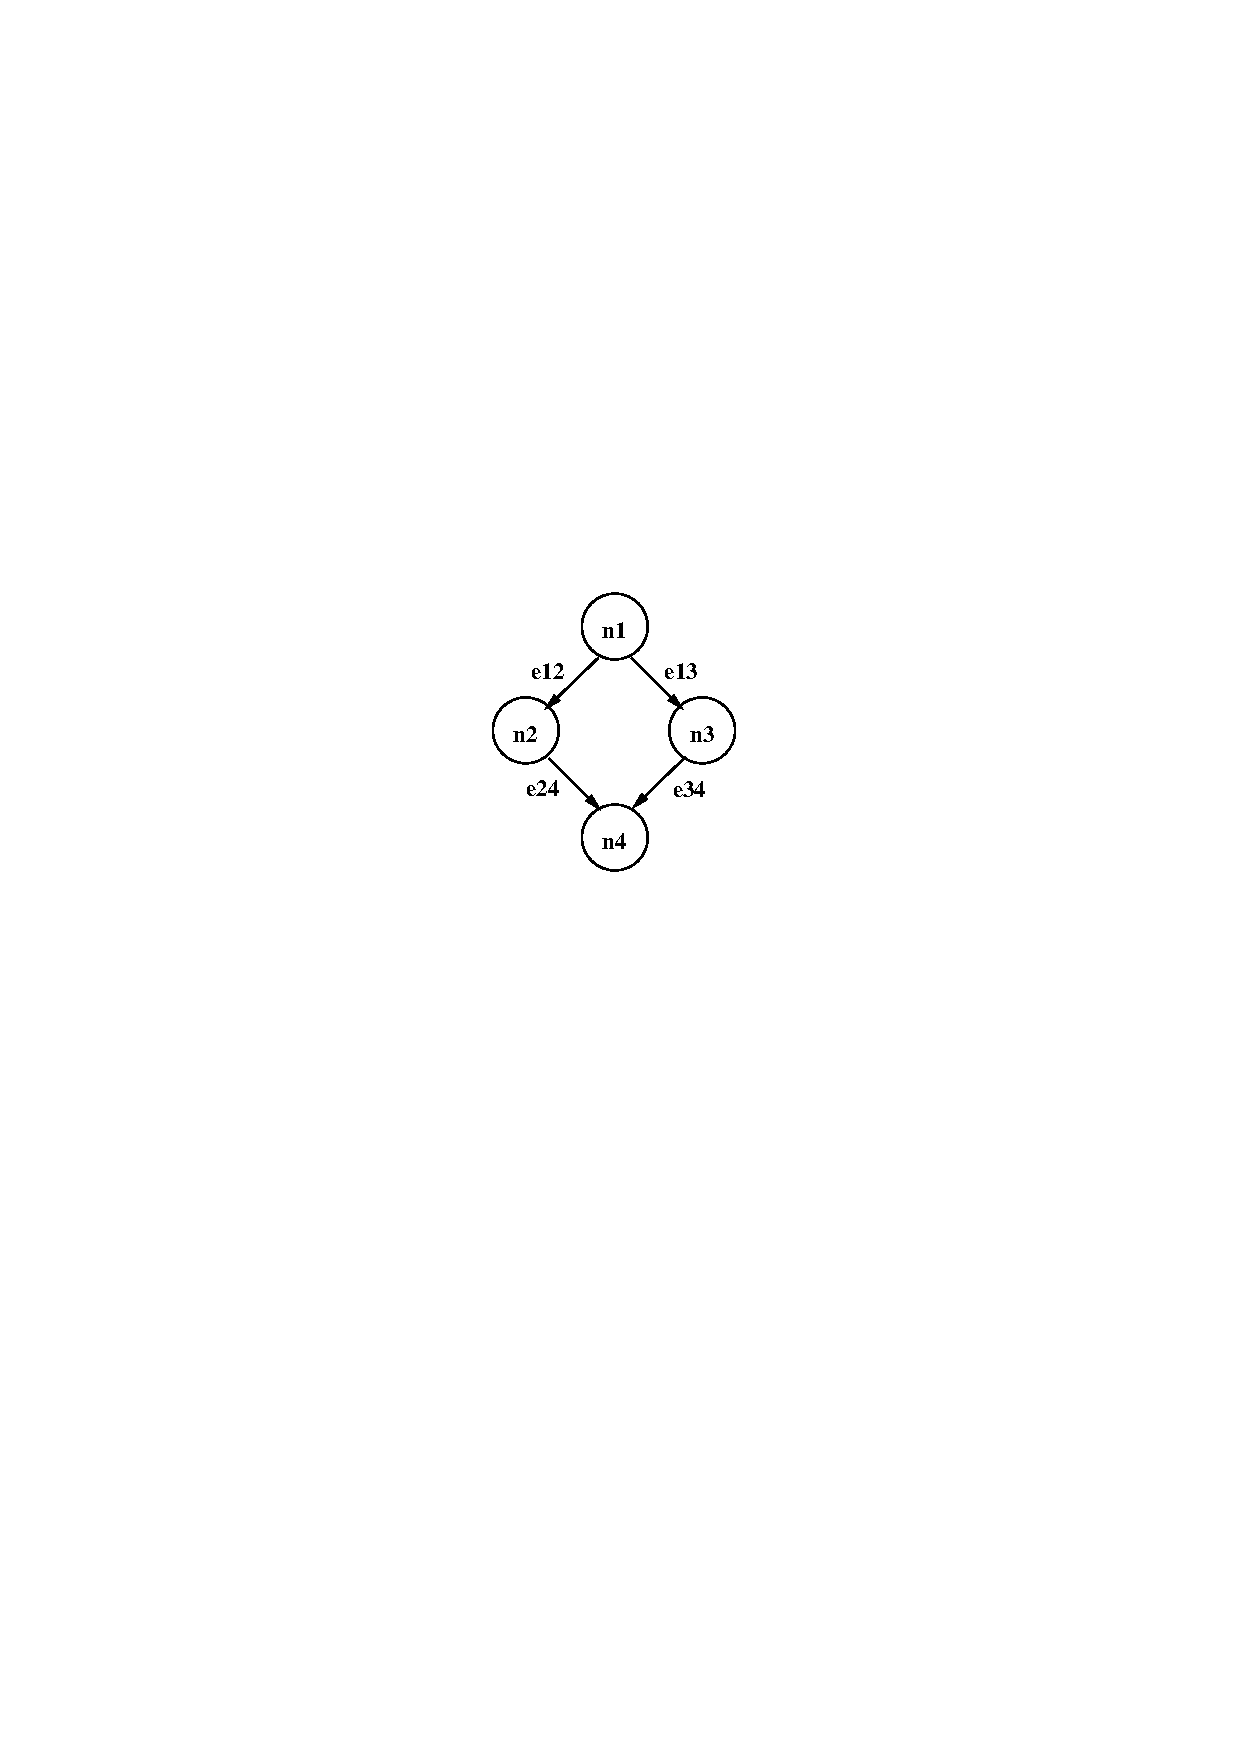
\includegraphics[height=1.25in]{acyclic.pdf}}
\end{minipage}
\end{tabular}
\end{center}
\caption{Acyclic Scalar Example}
\label{fig:acylic-scalar}
\end{figure}

\begin{figure}%[p]

%\begin{center}
%\parbox{3.0in}{
\begin{programa}
%\Tb $@i := (\;) ; @C := (\;) ; @k_1 := (\;)$ ; $@k_2 := (\;)$ \\
\mbox{n1:}\Tb $i := 1$ \\
%\Tb $@i := (1)$ \\

\Tb $C := i\ <\ n $ \\
%\Tb $@C := (1)$ \\
\Tb if $C$ then \\
\mbox{n2:}\Tc $k_1 :=  2\ *\ i$ \\
%\Tc $@k_1 := (1)$ \\
\Tb else \\
\mbox{n3:}\Tc $k_2 := 2\ *\ n$ \\
%\Tc $@k_2 := (1)$ \\
\Tb endif \\
\mbox{n4:} \Tb $k_3 := \phi(k_1,k_2)$ \\
%\Tb $@k_3 := max(@k1,@k2)$ \\
\Tb print $k_3$ \\
\end{programa}
%}
%\end{center}

\caption{Partial Array SSA form for the Acyclic Scalar Example}
\label{fig:ssa-acylic-scalar}
\end{figure}


\begin{figure}%[p]
%\begin{center}
%\parbox{3.0in}{
\begin{programa}
\Tb $\L(i) = \L(1)$ \\
%\Tb $\L(@i) = X_{n1}$ \\
\Tb $\L(C) = \L_{<}(\L(i),L(n)) $ \\
%\Tb $\L(@C) = X_{n1}$ \\
\Tb $\L(k_1) =  \L_{*}(\L(2), \L(i))$ \\
%\Tb $\L(@k_1) = X_{n2}$ \\
\Tb $\L(k_2) = \L_{*}($\L(2),\L(n)) \\
%\Tb $\L(@k_2) = X_{n3}$ \\
\Tb $\L(k_3) = \L_{\Phi}(\L(k_1), X_{e24}, \L(k_2), X_{e34})$ \\
%\Tb $\L(@k_3) =  \L_{max}(\L(@k1),\L(@k2))$ \\
\end{programa}
%}
%\end{center}

\caption{Equations for Assignments}
\label{fig:equations-assignments}
\end{figure}

\begin{figure}%[p]
%\begin{center}
%\parbox{3.0in}{
\begin{programa}
\Tb $X_{n1} = \True $ \\
\Tb $X_{n2} = X_{e12} $ \\
\Tb $X_{n3} = X_{e13} $ \\
\Tb $X_{n4} = X_{e24} \sqcap X_{e34} $ \\
\end{programa}
%}
%\end{center}
\caption{Equations for Nodes}
\label{fig:equations-nodes}
\end{figure}


\begin{figure}%[p]
%\begin{center}
%\parbox{3.0in}{
\begin{programa}
\Tb $X_{e12} = \L_{\T}(X_{n1},\L(C)) $ \\
\Tb $X_{e13} = \L_{\F}(X_{n1},\L(C)) $ \\
\Tb $X_{e24} = X_{n2}$  \\
\Tb $X_{e34} = X_{n3} $ \\
\end{programa}
%}
%\end{center}
\caption{Equations for Edges}
\label{fig:equations-edges}
\end{figure}



Let us first consider how the algorithm in
figure~\ref{fig:scc-alg} will work for the simple case of acyclic scalar code.  Consider the example program shown in figure~\ref{fig:acylic-scalar}. The
basic
blocks are labeled
$n1$, $n2$, $n3$ and $n4$. Edges $e12$, $e13$, $e24$ and
$e34$ connect nodes in the obvious way. The control flow
following block $n1$ depends on the value of variable
$n$. 
\REM{We will examine two
cases, one where $n$ is the constant value 10 and one where it is not
constant. In the first case control will always follow edge $e12$. In
the second case control can proceed along either branch. The algorithm
will determine that in the first case the value of $k$ in block $n4$
is a constant and that in the second case it is not.
}


The first step is to transform the example in
figure~\ref{fig:acylic-scalar} to partial
Array SSA form (with no @ variables) as shown in
figure~\ref{fig:ssa-acylic-scalar}. Note that since $k$ had
multiple assignments in the original program, a $\phi$ function is
required to compute $k_3$ as a function of $k_1$ and $k_2$. 



\REM{
\begin{figure}%[t]
\begin{center}
\begin{tabular}{ll} \\
Initial State: \\
$\L(i)$ = 1 & \\
%$\L(@i)$ = $\Maybe$  & \\
$\L(C)$ = $\True$  &
%$\L(@C)$ =  $\Maybe$  & \\
  $\Rightarrow$ reevaluation of $X_{e12}$ and $X_{e13}$. \\
$X_{e12}$ = $\Maybe$ & \\
$X_{e13}$ = $\No$ & \\
 & $\Rightarrow$ reevaluation of $X_{n2}$ and $X_{n3}$. \\
$X_{n2}$ =  $\Maybe$ & \\
$X_{n3}$ =  $\No$ & \\
 & $\Rightarrow$ reevaluation of$\L(k_1)$,   $X_{e24}$ \\
$\L(k_1)$ = 2 \\
%$\L(@k_1)$ =  $\Maybe$ \\
$X_{e24}$ = $\Maybe$ \\
 & $\Rightarrow$ reevaluation of
$X_{n4}$.  \\
$X_{n4}$ = $\Maybe$ \\
 & $\Rightarrow$ reevaluation of $\L(k_3)$. \\
$\L(k_3)$ = 2 
%$\L(@k_3)$ = $\Maybe$ \\
 & No more changes.
\end{tabular}
\end{center}
\caption{Trace of the algorithm when $n$ is a constant.}
\label{fig:trace-const}
\end{figure}



\begin{figure}%[t]
\begin{center}
\begin{tabular}{ll} \\
Initial State: \\
$\L(i)$ = 1  \\
%$\L(@i)$ = $\Maybe$  \\
$\L(C)$ = $\bot$ \\
%$\L(@C)$ =  $\Maybe$ \\
 &  $\Rightarrow$ reevaluation of $X_{e12}$ and $X_{e13}$.   \\
$X_{e12}$ = $\Maybe$ \\
$X_{e13}$ = $\Maybe$ \\
 &  $\Rightarrow$ evaluation of  $X_{n2}$ and $X_{n3}$. \\
$X_{n2}$ =  $\Maybe$ \\
$X_{n3}$ =  $\Maybe$ \\
 & $\Rightarrow$ reevaluation of $\L(k_1)$, $X_{e24}$,
$\L(k_2)$, $X_{e34}$.  \\
$\L(k_1)$ = 2 \\
%$\L(@k_1)$ =  $\Maybe$ \\
$X_{e24}$ = $\Maybe$ \\
$\L(k_2)$ = $\bot$ \\
%$\L(@k_2)$ =  $\Maybe$ \\
$X_{e34}$ = $\Maybe$ \\
 & $\Rightarrow$ reevaluation of $X_{n4}$.  \\
$X_{n4}$ = $\Maybe$ \\
 &  $\Rightarrow$  reevaluation of $\L(k_3)$.  \\
$\L(k_3)$ = $\bot$ \\
%$\L(@k_3)$ =  $\Maybe$ \\
 & No more changes.  \\
\end{tabular}
\end{center}
\caption{Trace of the algorithm when $n$ is not a constant.}
\label{fig:trace-not-const}
\end{figure}
}


The second step is to use the partial Array SSA form to create a set of
data-flow equations on lattice values for use by our constant
propagation algorithm.
The conversion to equations is performed as follows.
There is one equation created for each assignment statement in the program.
There is one equation created for each node in the CFG.
There is one equation created for each edge in the CFG.
The equations for the assignments in our example are shown in
figure~\ref{fig:equations-assignments}. 
The equations for the nodes and edges in our example are found in
figures~\ref{fig:equations-nodes} and \ref{fig:equations-edges} respectively.
\REM{
They follow from the lattice mapping rules for CFG nodes and edges discussed
in section~\ref{sec:arraylattice}.
There are two things
worth noting about the equations for assignments in figure~\ref{fig:equations-assignments}:
\begin{enumerate}
\item
The RHS of the assignments to @ variables are replaced in the
data-flow equations by the
execution flags of the block which contains them. The purpose of the
@ variables is to determine exactly when each assignment is
executed. If a regular variable is assigned a constant value, we
maintain the information that its value is constant even if the
assignment may not execute. With the @ variable, however, it is
exactly the question of whether or not the assignment is executed that
we aim to capture. For example, the data-flow
equation for assignment $@k_2 := (1)$ in
block $n3$ is $\L(@v) = X_{n3}$, where $X_{n3}$ is the executable flag
for block $n3$.

\item
\end{enumerate}
}


The lattice operations $\L_{<}$, $\L_{*}$, and
$\L_{max}$ use specific knowledge of their operation as well as the
lattice values of their operands to compute resulting lattice
operations. For example, $\L_{*}(\bot,\L(0))$ results in $\L(0)$
because the result of multiplying 0 by any number is 0.  




Next, we employ the work-list algorithm shown in figure~\ref{fig:scc-alg}, 
which reevaluates the equations until there are no further
changes.  A solution to the data-flow equations identifies
lattice values for each variable in the Array SSA form of the program, and for each node executable flag and
edge executable flag in the CFG.
Reevaluation of an equation associated with an
assignment may cause equations associated with other assignments to be
inserted on the work list. If the value appears in a conditional
expression, it may cause one of the equations associated with edges to
be inserted on the work list. Reevaluation of an edge's executable
flag may cause an equation
for a destination node's executable flag to
be inserted on the work list. If reevaluation of a node's executable flag indicates that
the node may be evaluated, then the equations associated with
assignments within that node to be added to the work list.
When the algorithm terminates, the lattice values for variables identify
the constants in the program, and  the lattice values for executable
flags of nodes identify
unreachable code.


\REM{
We now describe how our example program 
is processed by this algorithm. 
The initial state is that $\L(X_{n1}) = \Maybe$\footnote{Even though the
compiler knows that node $n1$ {\it must} be executed, we do not
make any distinction between the
$\Must$ and $\Maybe$ cases.  Making such a distinction in our constant
propagation algorithm can only increase compile-time without improving precision.  However, the distinction might be useful in future work
on other analysis algorithms
that use Array SSA form.}. The work list contains
the first four equations from figure~\ref{fig:equations-assignments},
all of which are associated with CFG node $n1$.
As mentioned earlier,
we will
examine two cases. Figure~\ref{fig:trace-const} traces the algorithm
in the case where $n$ equals the constant 10.
Figure~\ref{fig:trace-not-const} traces the algorithm
in the case where $n$ is not a constant.
}

Even though we assumed an acyclic CFG in the above discussion,
the algorithm in figure~\ref{fig:scc-alg} can be used unchanged for
performing constant propagation analysis on a CFG that may have
cycles.  The only difference is that the CFG may now contain
back edges. Each back edge will be evaluated when its source
node is modified. The evaluation of this back edge may result in the
reevaluation of its target node.

As in past work, it is easy to show that the
algorithm must take at most $O(Q )$ time, where
$Q$ is the number of data-flow equations, assuming that
the maximum arity
of a function is constant
and the maximum height
of the lattice is constant. 
This time does not include the cost for the computation of $\DS$ and
$\DD$ used for non-constant indices. The complexity of  $\DS$ and
$\DD$ varies with the precision desired.


\begin{figure}%[p]
% TODO: decided how to initialize \L(@A_0)?
\begin{eqnarray*}
\L(A_0) & = & \bot \\
%\L(@A_0) & = & \bot \\
\L(i) & = & \L(1) \\
%\L(@i) & = & X_{n1} \\
\L(C) & = & \L_{<}(\L(i),\L(n))  \\
%\L(@C) & = & X_{n1} \\
\L(k) & = & \L_{*}(\L(2), \L(i)) \\
%\L(@k) & = & X_{n2} \\
\L(A_1) & = & \L_{d[\:]}(\L(k), \L(i)) \\
%\L(@A_1) & = & \L_{d@[\:]}(\L(k), X_{n2} ) \\
%\L(A_2) & = & \L_{d\Phi}(\L(A_1), \L(@A_1), \L(A_0), \L(@A_0)) \\
\L(A_2) & = & \L_{d\phi}(\L(A_1), \L(A_0)) \\
%\L(@A_2) & = & \L_{@max}(\L(@A_1),\L(@A_0)) \\
%\L(A_3) & = & \L_{\Phi}(\L(A_2), \L(@A_2), \L(A_1), \L(@A_1)) \\
\L(A_3) & = & \L_{\Phi}(\L(A_2), X_{e24}, \L(A_0), X_{e14}) \\
%\L(@A_3) & = & \L_{@max}(\L(@A_2),\L(@A_1)) \\
\end{eqnarray*}
\caption{Equations for Assignments from figure \protect{\ref{fig:ssa-acyclic-array}}}
\label{fig:equations-array}
\end{figure}


As an example with array variables, figure~\ref{fig:equations-array} lists the data-flow
equations for the assignment statements in the Array SSA program in
figure~\ref{fig:ssa-acyclic-array} (the data-flow equations for nodes
and edges are omitted, since they
simply follow the CFG structure).
Given the definition of lattice elements for
array variables from section~\ref{sec:arraylattice},
the conditional constant propagation algorithm
in figure~\ref{fig:scc-alg} can basically be used unchanged for  
array variables.

\REM{The main extension is the introduction of new transfer functions that are 
necessary for computing lattice elements arising from 
array references --- $\L_{d[\:]}$, $\L_{d@[\:]}$, $\L_{d\Phi}$, $\L_{@max}$,
$\L_{\Phi}$.
The function tables for these transfer functions are shown in
figures~\ref{fig:adef}, \ref{fig:@def}, \ref{fig:dphi}, \ref{fig:@max},
and \ref{fig:Phi}
respectively.
In addition, figure~\ref{fig:aref} shows the transfer function for
an array reference operator, which is needed  to 
replace array references $A_2[k]$ and $A_3[2]$ 
in figure~\ref{fig:ssa-acyclic-array}
by constants, after a solution to the equations has been obtained.

Note that the value of
$\L(A_2)  =  \L_{d\Phi}(\L(A_1), \L(@A_1), \L(A_0), \L(@A_0))$
in figure~\ref{fig:dphi} does not depend on $\L(@A_1)$ and
$\L(@A_0)$.  
% Why?  Because A_1 only updates a single element and we only consider
% two cases for an @ array element, NO and MAYBE?
However, the values of $\L(@A_1)$ and
$\L(@A_0)$ do feed into $\L(@A_2)  =  \L_{@max}(\L(@A_1),\L(@A_0))$.

}


